\begin{vkrthesis}%
	{Анализ и применение многофакторных моделей динамики лекарственных средств в медицинских исследованиях}%
	{Лазар~В.\,И.}%
	
	\VKRAuthorDetailsSupervisorConsultant%
	{Лазар Владислав Игоревич}%
	{Кафедра математической статистики}%
	{vlad.lazar.ik528@yandex.ru}%
	{Захарова Татьяна Валерьевна}%
	{к.ф.-м.н.}%
	{доц.}%
	{}%
	{}
	{}%
	{}%
	
	% Здесь можно для удобства переопределить некоторые команды
	\newcommand{\tbs}{\textbackslash}
	\newcommand{\todo}[1]{\textcolor{red}{#1}}
	
	В работе рассматривается задача проверки лекарственных препаратов на биоэквивалентность. Исследования биоэквивалентности лежат в основе воспроизведения лекарственных препаратов, подтвердивших свою эффективность и безопасность. Основным методом проверки гипотезы биоэквивалентности является процедура двух односторонних тестов Шуирманна. Она используется в течение многих лет и подтвердила свою пригодность для доказательства эквивалентной биодоступности.
	\par
	В исследованиях биоэквивалентности одной из использующихся сравнительных характеристик лекарств является площадь под кривой (AUC) <<концентрация—время>>. Основной проблемой классического критерия является нечувствительность к форме этой кривой, что может влечь за собой некорректную оценку действия воспроизведенного лекарства.
	\par
	Авторами предложен новый подход в оценке параметров исследуемых лекарств. В качестве основы берётся оценка траектории с помощью математической модели \textbf{PBFTPK}. В оригинальной статье предлагается оценка параметров модели по конечному числу наблюдений методом минимизации среднеквадратичной функции потерь. В работе представлены модификации оригинальной модели устойчивые к проблемам возникающим в реальных данных - неравномерности наблюдений по времени и наличию более одного пика траектории. Неоднородность наблюдений влечёт за собой уменьшение значимости более редких наблюдений и как следствие худшее качество модели на соответствующих участках. В случае многих пиков классические алгоритмы рассматривают побочные пики как шум в данных, вследствие чего теряется важная для пролонгированных форм информация о действии лекарства.
	\par
	На начальном этапе исследований проводилась оценка траектории с помощью оригинальной модели. Методом последовательного квадратичного программирования (\textbf{SLSQP}) проводилась оценка параметров следующей параметризованной функции:
	\[
		\begin{cases}
			C(t) = \frac{F D}{V_d} \frac{e^{-k_{el}t} - e^{k_a t}}{k_a - k_{el}}, & 0 \leq t \leq \tau, \\
			C(t) = C(\tau) e^{-k_{el} (t - \tau)},                                & \tau < t < +\infty
		\end{cases}
	\], где
	\begin{itemize}
		\item $F$ - биодоступная доля дозы
		\item $D$ - доза вещества
		\item $V_d$ - объём распределения вещества
		\item $k_a$ - коэффициент абсорбции
		\item $k_{el}$ - коэффициент элиминации
	\end{itemize}
	Для дальнейшей работы важно выделить два этапа - этап абсорбции ($t \leq \tau$) и этап элиминации ($t > \tau$).
	\par
	Для устранения первой проблемы авторами предложен метод взвешивания функции потерь в соответствии с фазой действия лекарственного вещества. Для этого рассматривается $\lambda$-взвешенная среднеквадратичная функци потерь ($\textbf{WMSE}_{\lambda}$):
	
	\[
		L_{\lambda}(t, C, \hat{C}) = \frac{1}{\#(t)}\sum_{t_i \in t} \Big(C(t_i)-\hat{C}(t_i)\Big)^2 \cdot
		\begin{cases}
			1,       & t_i \le \tau \\
			\lambda, & t_i > \tau
		\end{cases}
	\]
	
	Такой метод взвешивания объясняется особенностями используемых данных, а конкретно -- малой длительностью фазы абсорбции относительно фазы элиминации и большей плотностью наблюдений именно на этапе абсорбции.
	\begin{figure}[h!]
		\center
		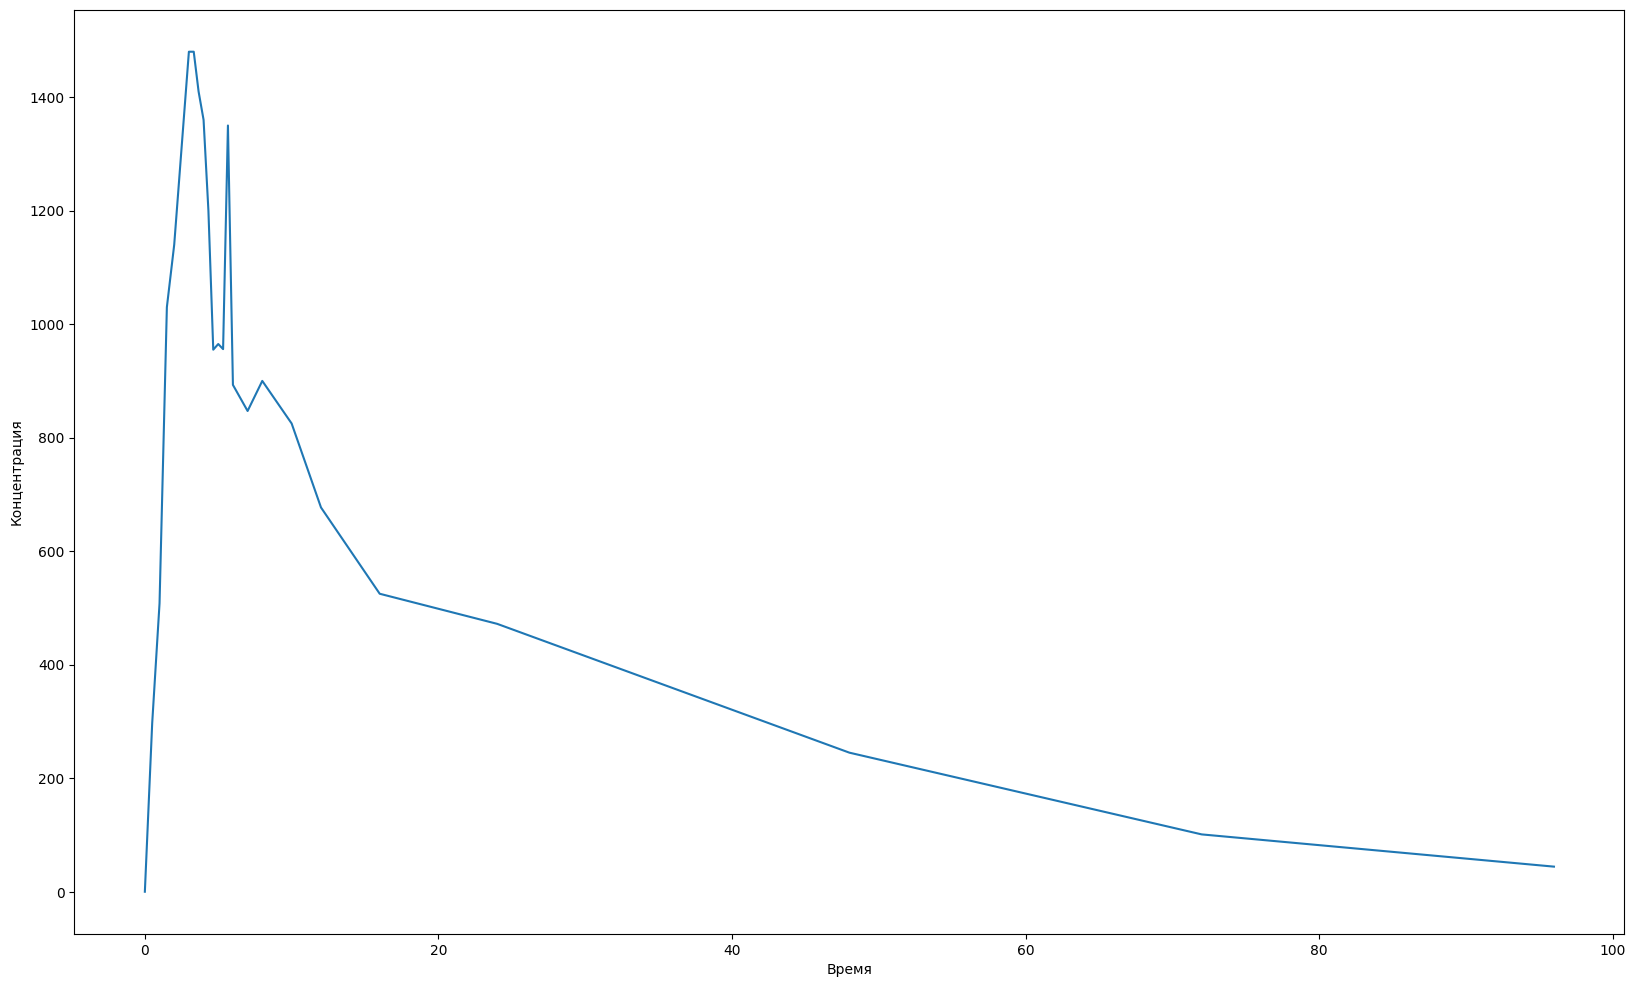
\includegraphics[width=1.0\linewidth]{img/sample.png}
		\caption{Пример данных для исследования}
		\label{fig:comparison}
	\end{figure}
	\par
	Для сохранения информации о множественных пиках траектории был предложен метод ансмаблирования математических моделей. Под ансмаблированием понимается следующий алгоритм действий:
	\begin{enumerate}
		\item Задаётся размер ансамбля - количество базовых моделей.
		\item На вход первой модели для оценивания подаются данные.
		\item Вычисляется разность оценивания и исходных данных, такую разность будем называть \textbf{остатком}.
		\item Полученный остаток подаётся на вход следующей модели в ансамбле, после чего процесс повторяется начиная с пункта 2.
	\end{enumerate}
	Помимо повышения точности оценивания (оценивание остатка модели вместо его отбрасывания) полученный алгоритм не теряет физической интерпретируемости. В данном случае каждую модель в ансамбле можно рассматривать как отдельную независимо действующую фракцию исходного вещества. Тогда полная оценка траектории получается как сумма оценок всех моделей в ансамбле, то есть концентрация вещества в крови есть сумма концентраций его частей, что соотносится с физическим смыслом исследуемого явления.
	\par Метод программно реализован на Python и оформлен в виде программного пакета (бибилиотеки). Проведено сравнение оригинального метода и модифицированного.
	
	\begin{figure}[!htb!]
		\minipage{0.5\linewidth}
		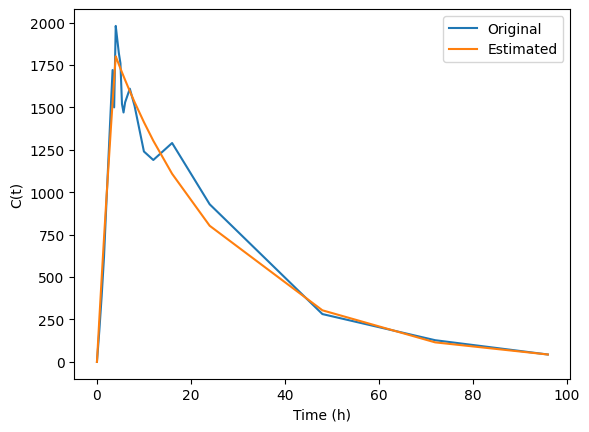
\includegraphics[width=1.0\textwidth]{img/results/basic_1.png}
		% \captio\cite{pbftpk}n{Оригинальный метод}
		\endminipage \hfill
		\minipage{0.5\linewidth}
		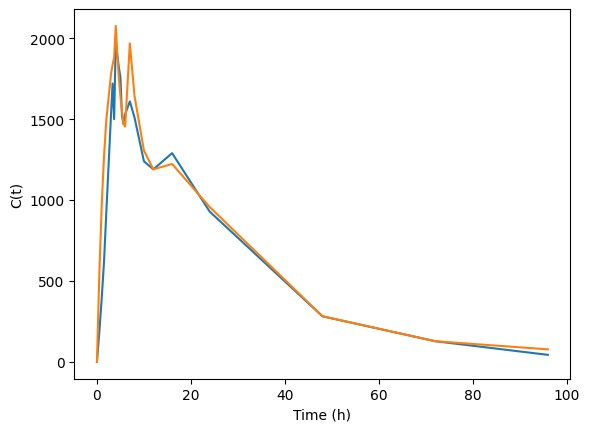
\includegraphics[width=1.0\textwidth]{img/results/1.jpg}
		% \caption{Модифицированный метод}
		\endminipage \hfill
	\end{figure}
	\begin{figure}[!htb!]
		\minipage{0.5\linewidth}
		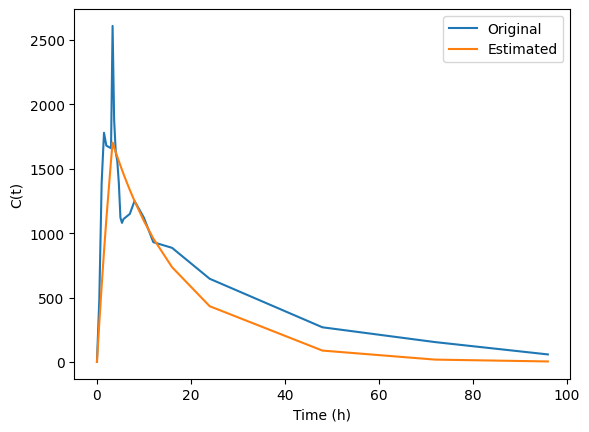
\includegraphics[width=1.0\textwidth]{img/results/basic_2.png}
		% \captio\cite{pbftpk}n{Оригинальный метод}
		\endminipage \hfill
		\minipage{0.5\linewidth}
		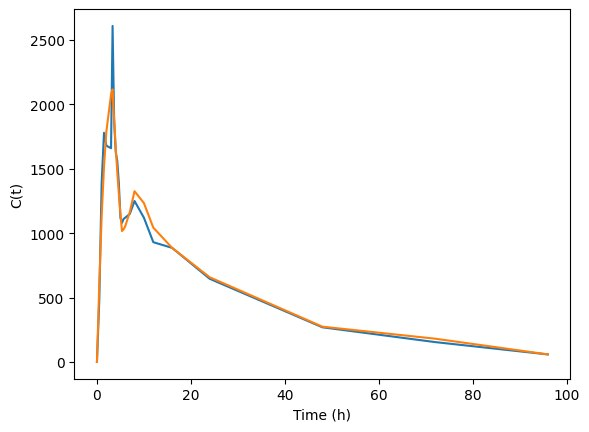
\includegraphics[width=1.0\textwidth]{img/results/2.jpg}
		% \caption{Модифицированный метод}
		\endminipage \hfill
	\end{figure}
	
	Как можно видеть, модифицированный метод справляется с поиском множественных пиков и проявляет себя лучше оригинального на <<хвостах>> оцениваемой траектории. Средняя квадратичная ошибка ансамблевого метода с взвешенными ошибками - 164.2, в то время как оригинальная модель имеет почти вдвое худший показатель качества - примерно 321.6.
	
	\par Полученный модифицированный метод позволяет не только более точно оценить форму кривой, но и перейти от сравнения исходных кривых к сравнению физически интерпретируемых показателей препарата (количество пиков, коэффициенты абсорбции и элиминации). Также это даёт возможность использовать другие методы анализа основанные на метрической близости объектов линейных пространств (например, кластерный анализ).
\end{vkrthesis}
